
\msection{MEWE: Multi-variant Execution for WebAssembly}
\label{section:mewe}

\renewcommand{\tool}{MEWE\xspace}
% Overview
This section describes MEWE \cite{MEWE}. 
\tool synthesizes diversified function variants by using CROW.
It then provides execution-path randomization in a Multivariant Execution (MVE) \cite{bhatkar03}.
Execution path randomization is a technique that randomizes the execution path of a program at runtime, i.e. at each invocation of a function, a different variant is executed.
MEWE generates application-level multivariant binaries without changing the operating system or \wasm\ runtime.
It creates an MVE by intermixing functions for which CROW generates variants, as illustrated by the green square in \autoref{fig:approach_landscape}.
\tool inlines function variants when appropriate, resulting in call stack diversification at runtime.



As illustrated in \autoref{workflow}, MEWE takes the LLVM IR variants generated by CROW's diversifier. 
It then merges LLVM IR variants into a Wasm multivariant.
In the figure, we highlight the two components of MEWE, \emph{Multivariant Generation} and the \emph{Mixer}.
In the \emph{Multivariant Generation} process, 
MEWE gathers the LLVM IR variants created by CROW.
The Mixer component, on the other hand, links the multivariant binary and creates a new entrypoint for the binary called \emph{entrypoint tampering}.
The tampering is needed in case the output of CROW are variants of the original entrypoint, e.g. the \emph{main} function.
Concretely, it wraps the dispatcher for the entrypoint variants as a new function for the final Wasm binary and is declared as the application entrypoint.
The random generator is needed to perform the execution-path randomization.
For the random generator, we rely on WASI's specification \cite{WASI} for the random behavior of the dispatchers. 
However, its exact implementation is dependent on the platform on which the binary is deployed. 
Finally, using the same custom Wasm LLVM backend as CROW, we generate a standalone multivariant \wasm\ binary.
Once generated, the multivariant \wasm\ binary can be deployed to any \wasm\ engine. 

\begin{figure*}
  \centering
  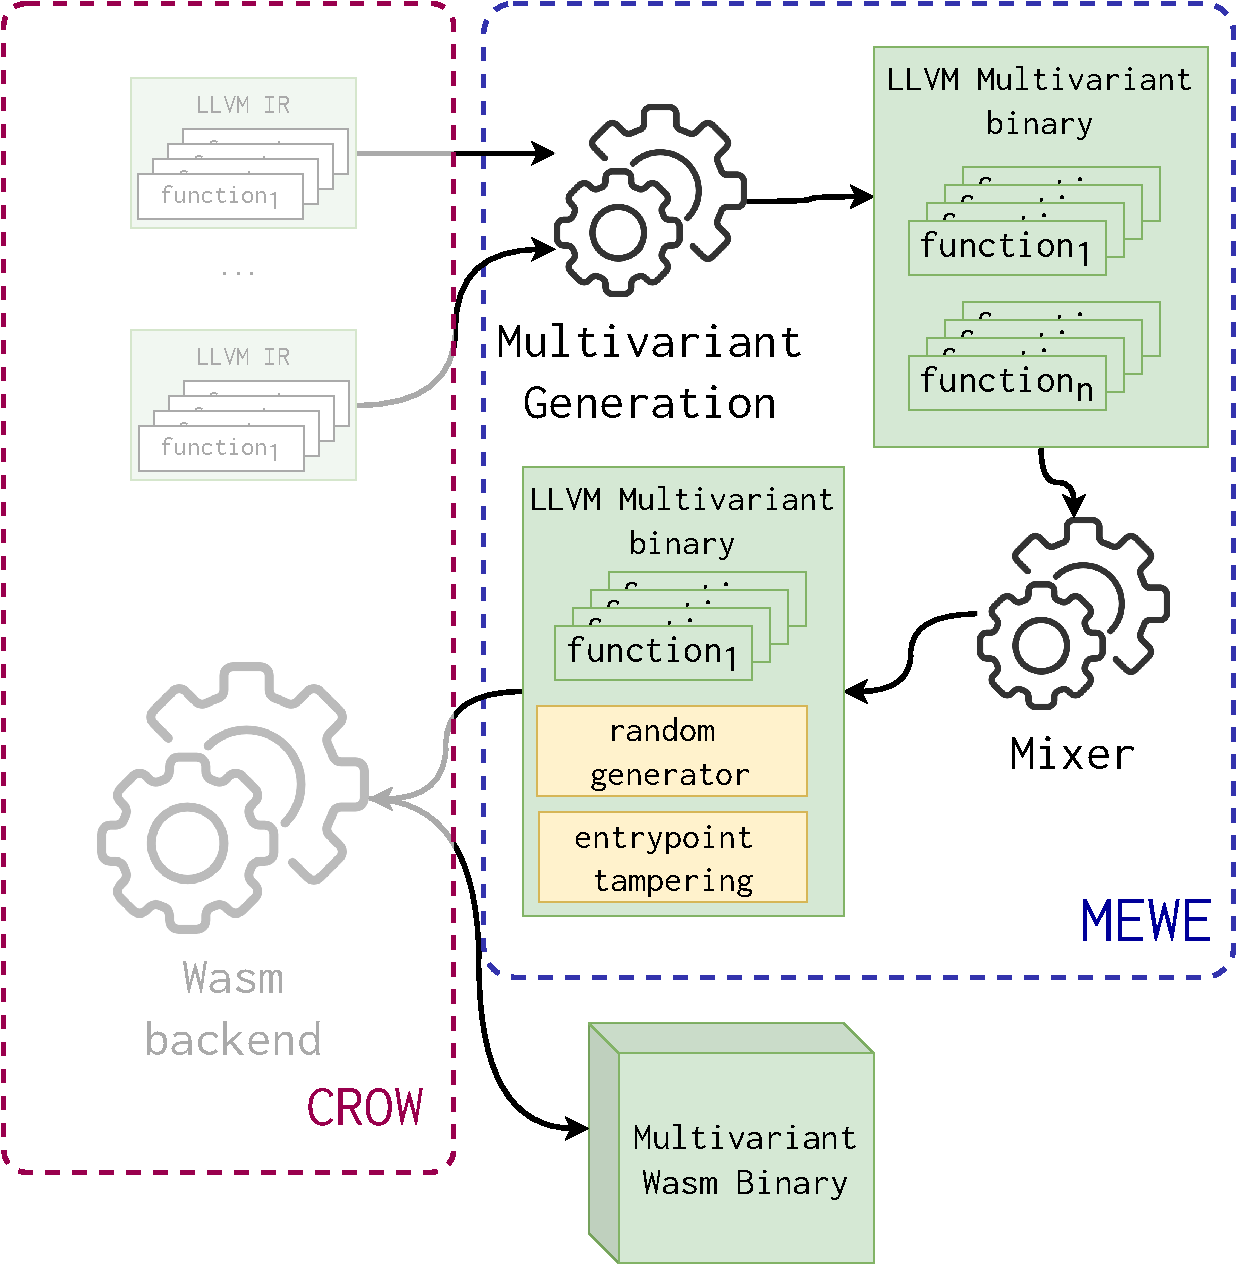
\includegraphics[height=3.2in]{diagrams/MEWE.pdf}
  \caption{Overview of \tool workflow. It takes as input an LLVM binary. It first generates a set of functionally equivalent variants for each function in the binary using CROW. Then, MEWE generates an LLVM multivariant binary composed of all the function variants. Finally, the Mixer includes the behavior in charge of selecting a variant when a function is invoked. Finally, the \tool mixer composes the LLVM multivariant binary with a random number generation library and tampers the original application entrypoint. The final process produces a \wasm\ multivariant binary ready to be deployed. }
  \label{workflow}
\end{figure*}

\msubsection{Multivariant call graph}

The key component of \tool consists of combining the variants into a single binary.
The core idea is to introduce one dispatcher function per original function with variants.
A dispatcher function is a synthetic function in charge of choosing a variant at random when the original function is called.
With the introduction of the dispatcher function,  \tool turns the original call graph into a multivariant call graph, defined as follows. 


\begin{definition}{Multivariant Call Graph (MCG):}\label{def:EP}
  A multivariant call graph is a call graph $\langle N, E \rangle$ where the nodes in $N$ represent all the functions in the binary and an edge $(f_1,f_2) \in E$ represents a possible invocation of $f_2$ by $f_1$  \cite{ryder1979}. The nodes in $N$ have three possible types: a function present in the original program,  a generated function variant, or a dispatcher function.
\end{definition}


 
\msubsection{Exemplifying a Multivariant binary}


% Instance of a multivariant module
In \autoref{multivariant}, we show the original static call graph for an original program (top of the figure), as well as the multivariant call graph generated with \tool (bottom of the figure).
The gray nodes represent function variants, the green nodes function dispatchers, and the yellow nodes are the original functions.
The directed edges represent the possible calls.
The original program includes three functions. \tool generates 43 variants for the first function, none for the second, and three for the third. 
\tool introduces two dispatcher nodes for the first and third functions. Each dispatcher is connected to the corresponding function variants to invoke one variant randomly at runtime.


\begin{figure}[h]
  \centering
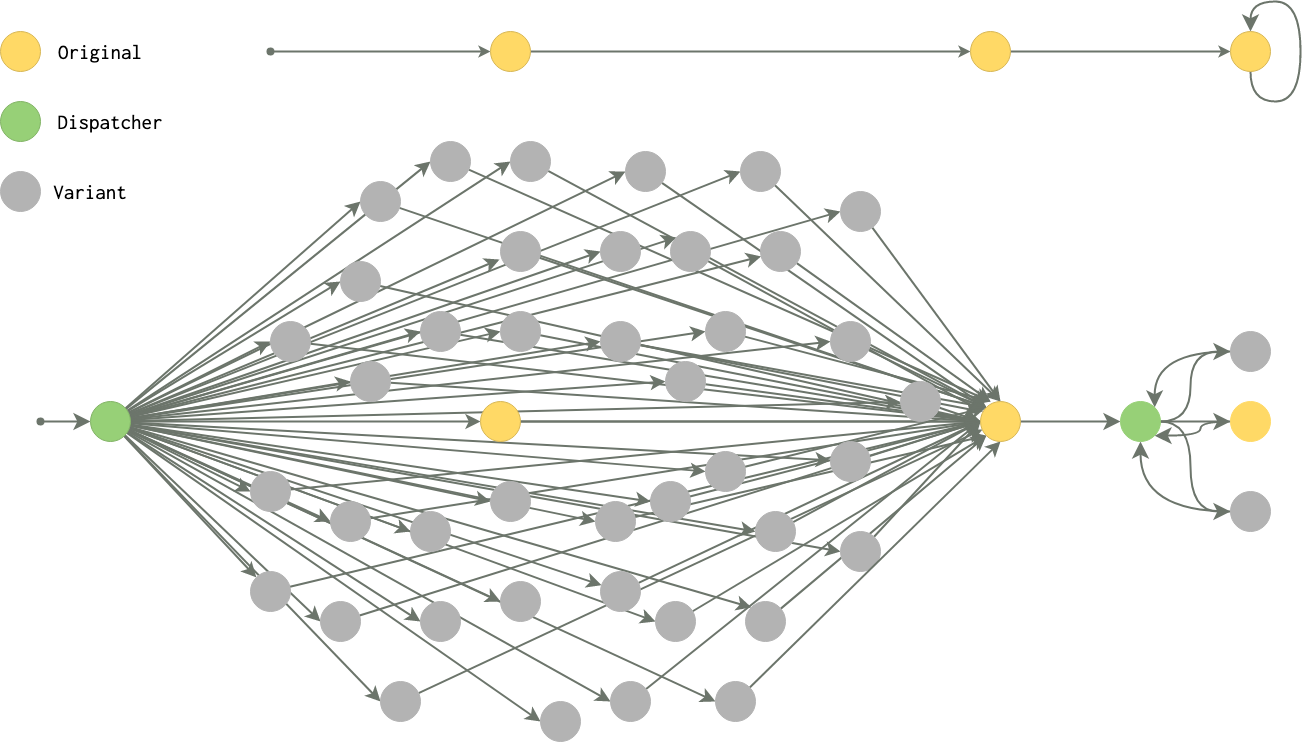
\includegraphics[width=.75\linewidth]{diagrams/CFG.png}
\caption{Example of two static call graphs. At the top, is the original call graph, and at the bottom, is the multivariant call graph, which includes nodes that represent function variants (in gray), dispatchers (in green), and original functions  (in yellow).
}
\label{multivariant}
\end{figure}

In \autoref{listing:multivariant_template}, we demonstrate how MEWE constructs the function dispatcher, corresponding to the rightmost green node in \autoref{multivariant}, which handles three created variants including the original. 
The dispatcher function retains the same signature as the original function. Initially, the dispatcher invokes a random number generator, the output of which is used to select a specific function variant for execution (as seen on line 6 in \autoref{listing:multivariant_template}). 
To enhance security, we employ a switch-case structure within the dispatcher, mitigating vulnerabilities associated with speculative execution-based attacks \cite{Narayan2021Swivel} (refer to lines 12 to 19 in \autoref{listing:multivariant_template}). 
This approach also eliminates the need for multiple function definitions with identical signatures, thereby reducing the potential attack surface in cases where the function signature itself is vulnerable \cite{johnson2021}.
Additionally, MEWE can inline function variants directly into the dispatcher, obviating the need for redundant definitions (as illustrated on line 16 in \autoref{listing:multivariant_template}). 
Remarkably, we prioritize security over performance, i.e., while using indirect calls in place of a switch-case could offer constant-time performance benefits, we implement switch-case structures.


\lstset{
    language=llvm,
    %style=nccode,
    basicstyle=\footnotesize\ttfamily,
    columns=fullflexible,
    breaklines=true,
    numbers=none,
    stepnumber=1,
    float
}

\begin{minipage}[t]{0.9\linewidth}
\scriptsize
\centering
\noindent\begin{minipage}[b]{\linewidth}
    \begin{minipage}[t]{1\linewidth}
        \begin{lstlisting}[escapeinside={(*}{*)}, numbers=left]
; Multivariant foo wrapping ;
define internal i32 @foo(i32 %0) {
    entry:
      ; It first calls the dispatcher to discriminate between the created variants ;
      %1 = call i32 @discriminate(i32 3)
      switch i32 %1, label %end [
        i32 0, label %case_43_
        i32 1, label %case_44_
      ]
    ;One case for each generated variant of foo ;
    case_43_:                 
      %2 = call i32 @foo_43_(%0)
      ret i32 %2
    case_44_:
      ; MEWE can inline the body of the a function variant ;
      %3 = <body of foo_44_ inlined>
      ret i32 %3
    end:                                  
      ; The original is also included ;           
      %4 = call i32 @foo_original(%0)
      ret i32 %4
}
        \end{lstlisting}
    \end{minipage}%
    
    \noindent\rule{\linewidth}{0.4pt}
    \captionof{lstlisting}{Dispatcher function embedded in the multivariant binary of the original function in the rightmost green node in \autoref{multivariant}. The code is commented for the sake of understanding. }\label{listing:multivariant_template}
\end{minipage}
\end{minipage}

In  \autoref{listing:multivariant_template}, we illustrate the LLVM construction for the function dispatcher corresponding to the right most green node of \autoref{multivariant}.
Notice that, the dispatcher function is constructed using the same signature as the original function. 
It first calls the random generator, which returns a value used to invoke a specific function variant (see line 6 in \autoref{listing:multivariant_template}). 
We utilize a switch-case structure in the dispatchers to prevent indirect calls, which are vulnerable to speculative execution-based attacks \cite{Narayan2021Swivel} (see lines 12 to 19 in \autoref{listing:multivariant_template}), i.e., the choice of a switch-case also avoids having multiple function definitions with the same signature, which could increase the attack surface in case the function signature is vulnerable \cite{johnson2021}.
In addition, MEWE can inline function variants inside the dispatcher instead of defining them again (see line 16 in \autoref{listing:multivariant_template}).
Remarkably, we trade security over performance since dispatcher functions that perform indirect calls, instead of a switch-case,  could improve the performance of the dispatchers as indirect calls have constant time.


%\msubsection{MEWE's Mixer}

%\todo{Augment the description of the MIXER.}



\begin{tcolorbox}[title=Contribution paper and artifact,boxrule=1pt,arc=.2em,boxsep=1.0mm]
  MEWE provides dynamic execution path randomization by packaging variants generated out of CROW.\\
  MEWE is fully presented in Cabrera-Arteaga \etal "Multi-Variant Execution at the Edge"
  \emph{Proceedings of Moving Target Defense, 2022, ACM}
 \url{https://dl.acm.org/doi/abs/10.1145/3560828.3564007}
 \\\\
 MEWE is also available as an open-source tool at \url{https://github.com/ASSERT-KTH/MEWE}
\end{tcolorbox}